\documentclass[
  babelLanguage=english,
  final,
  webversion,
  %showtrims,
]{chantingbook}

\usepackage{local}

\makeatletter

\newcommand{\verseref}[1]{\sidepar{#1}}

\definecolor{titlecolor}{gray}{0.1}

\makeatother

\title{Sumedharama Monastic Chants}

\begin{document}

\frontmatter

% Cover page

\thispagestyle{empty}\mbox{}
\AddToShipoutPictureFG*{%
  \put(\LenToUnit{-3mm},\LenToUnit{-3mm}){%
    \begin{minipage}[b][\paperheight + 6mm][c]{\paperwidth + 6mm}%
      \centering%
      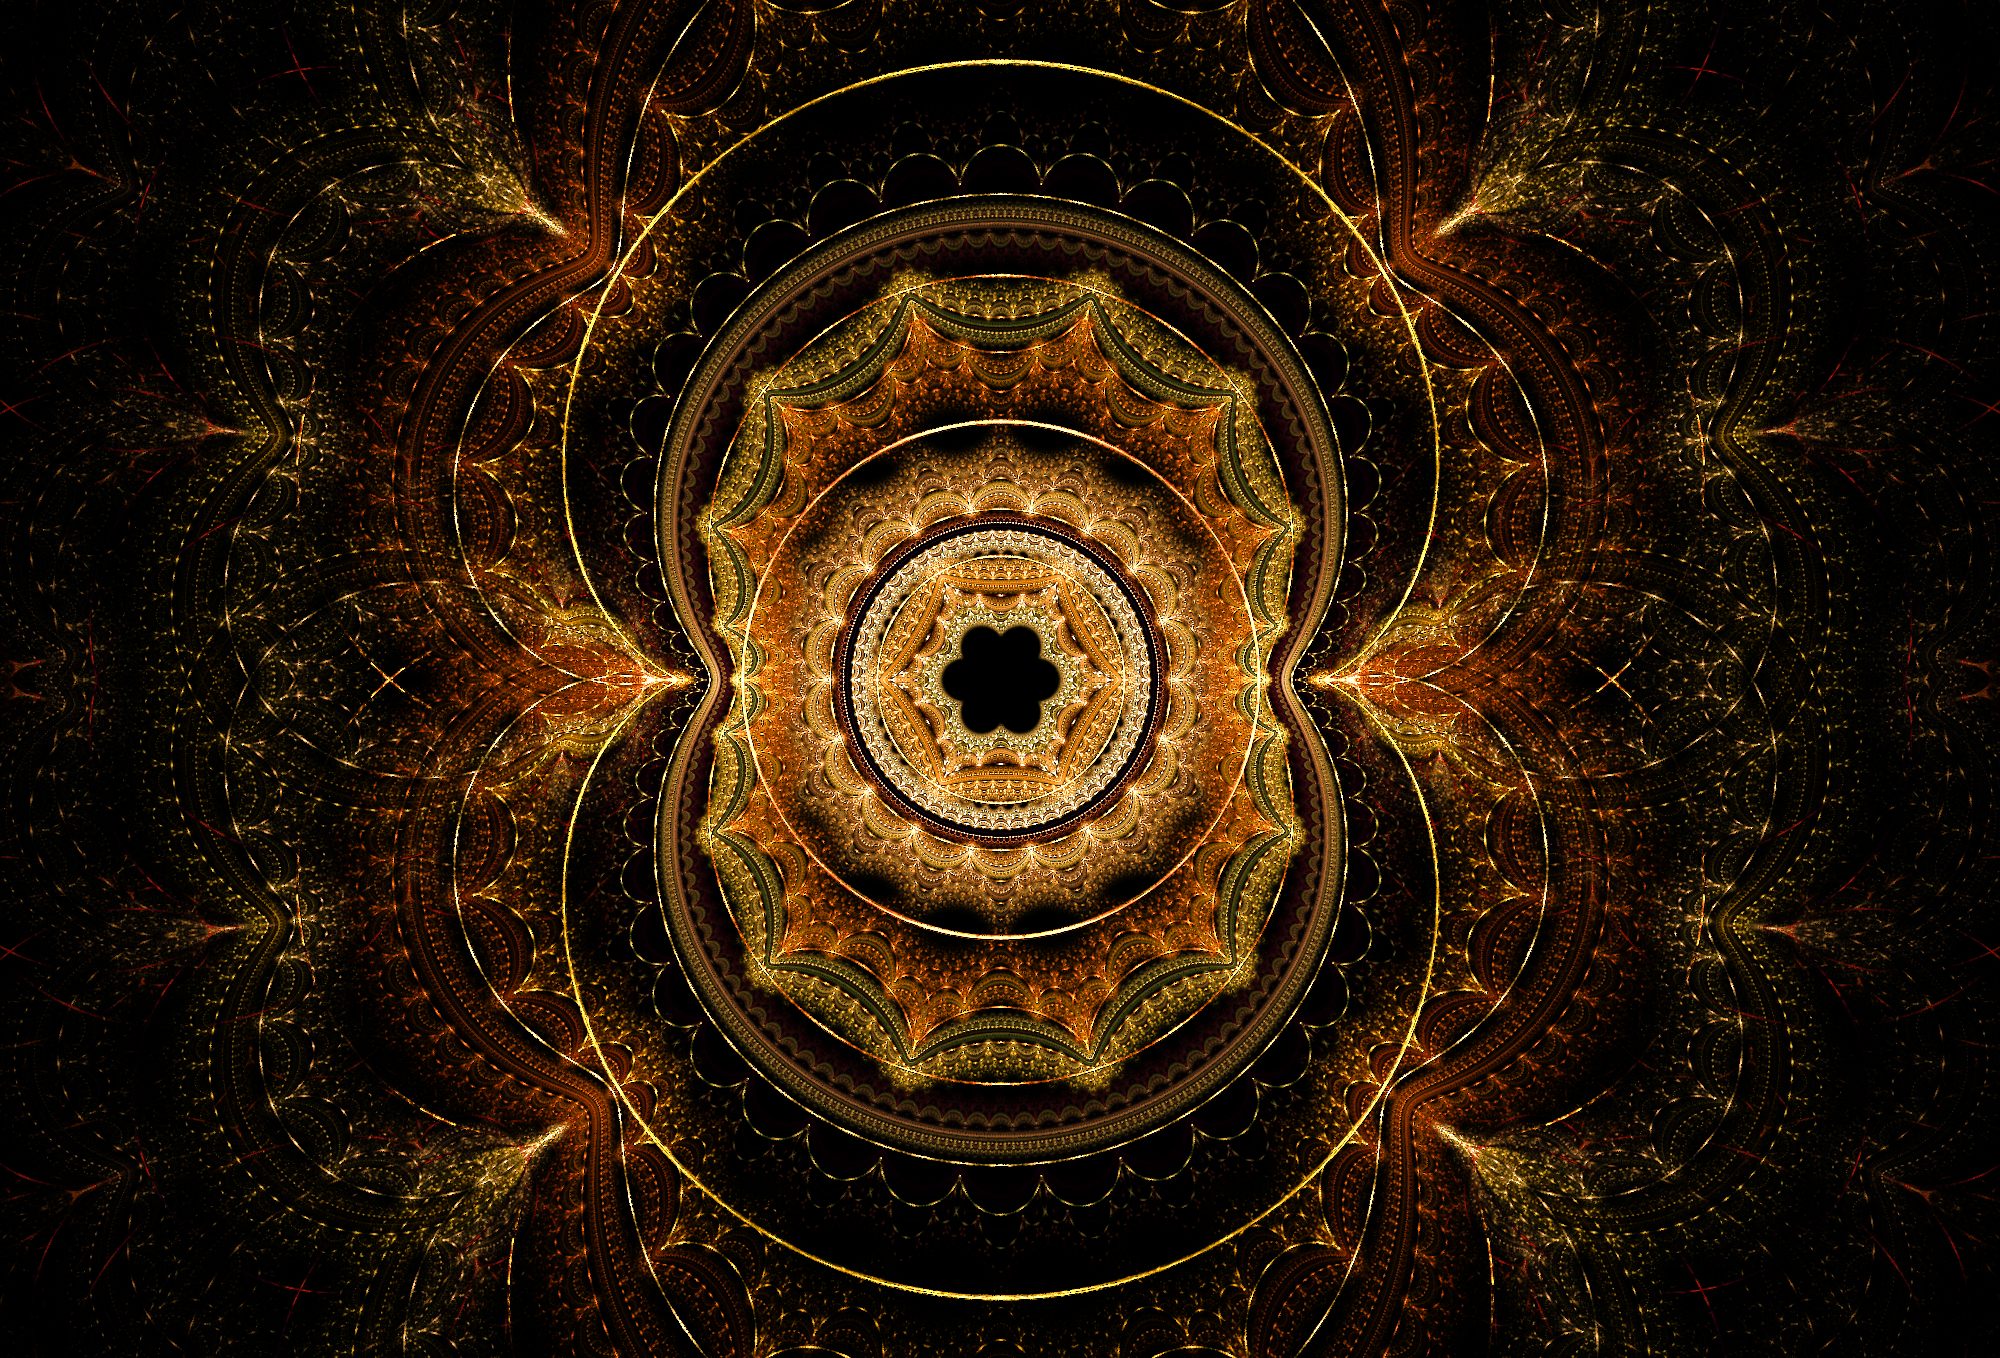
\includegraphics[width=\paperwidth+6mm]{inner-peace-crop}%
      \par%
      \vspace*{1cm}%
      \resizebox{70mm}{!}{\color{titlecolor}\Calluna\textls{CÂNTICOS}}%
      \par%
      \vspace*{2cm}%
    \end{minipage}%
  }%
}%
\clearpage

\cleartorecto
\tableofcontents*

\mainmatter

\usePsMarksTitleOnly

\chapter*[Partilha de Bençãos]{Reflexões sobre a Partilha de Bençãos}

\delegateSetUseNext

\begin{leader}
  [Ha꜓nda mayaṁ uddissanādhiṭṭhāna-gāthā꜓yo b꜕haṇāmase]
\end{leader}

\firstline{Iminā puññakammena upajjhāyā guṇuttarā}

[Iminā puñña꜕kammena] u꜕pajjhāyā gu꜕ṇutta꜕rā\\
Ācariyūpa꜕kārā ca꜕ mātāpitā ca꜕ ñāta꜕kā\\
Suriyo candimā rājā gu꜕ṇavantā na꜕rāpi꜕ ca꜕\\
Brahma-mārā ca꜕ indā ca꜕ loka꜕pālā ca꜕ deva꜕tā\\
Yamo mittā ma꜕nussā ca majjhattā veri꜕kāpi꜕ ca꜕\\
Sa꜕bbe sattā sukhī hontu puññāni pa꜕ka꜕tāni꜕ me\\
Sukhañca tividhaṁ dentu꜕ khippaṁ pāpetha꜕ voma꜕taṁ\\
Iminā puññakammena iminā uddi꜕ssena꜕ ca꜕\\
Khipp'āhaṁ su꜕la꜕bhe ceva taṇhūpādāna꜕-cheda꜕naṁ\\
Ye santāne hīnā dhammā yāva꜕ nibbāna꜕to ma꜕maṁ\\
Nassantu sabba꜕dā yeva yattha꜕ jāto bha꜕ve bha꜕ve\\
Ujucittaṁ sa꜕ti꜕paññā sallekho vi꜕ri꜕yamhinā\\
Mārā labhantu nokāsaṁ kātuñca vi꜕ri꜕yes꜕u me\\
Buddhādhipa꜕va꜕ro nātho dhammo nātho va꜕rutta꜕mo\\
Nātho pacceka꜕buddho ca꜕ saṅgho nāthotta꜕ro ma꜕maṁ\\
Tesottamānubhāvena mārokāsaṁ la꜕bhantu꜕ mā

\chapter[Partilha de Bençãos]{Reflexões sobre a Partilha de Bençãos}

\enlargethispage{2\baselineskip}

\begin{leader}
  [Cantemos agora as Reflexões sobre a Partilha de Bençãos]
\end{leader}

\firstline{Através do bem que resulta da minha prática}

Através do bem que resulta da minha prática,\\
Que os meus mestres e guias espirituais de grande virtude,\\
A minha mãe, o meu pai e os meus familiares,\\
O Sol e a Lua, e todos os líderes virtuosos do mundo,\\
Que os Deuses mais elevados e as forças do mal,\\
Seres celestiais, espíritos guardiões da Terra e o Senhor da Morte,\\
Aqueles que são amigáveis, indiferentes ou hostis,\\
Que todos os seres recebam as bênçãos da minha vida.\\
Que brevemente cheguem à Tripla Bênção, e superem a morte.

Através do bem que resulta da minha prática,\\
E através desta partilha,\\
Que todos os desejos e apegos rapidamente cessem\\
Assim como os estados prejudiciais da mente.

Até realizar o Nibbana,\\
Em qualquer tipo de nascimento, que eu tenha uma mente justa,\\
Com consciência e sabedoria, austeridade e vigor.\\
Que as forças ilusórias não controlem,\\
nem enfraqueçam a minha decisão.

O Buddha é o meu excelente refúgio,\\
Insuperável é a proteção do Dhamma,\\
O Buddha solitário é o meu Nobre exemplo,\\
O Saṅgha é o meu maior suporte.

Que através desta supremacia\\
Desapareçam a escuridão e a ilusão.

\chapter*[Metta Sutta]{Metta Sutta}

\delegateSetUseNext

\firstline{Karaṇīyam-attha-kusalena}

\begin{leader}
  [Ha꜓nda mayaṁ metta-sutta-gāthā꜓yo bha꜕ṇāmase]
\end{leader}

[Karaṇīyam-attha-kusalena]\\
Yan-taṁ santaṁ padaṁ abhisamecca\\
Sakko ujū ca suhujū ca\\
Suvaco c'assa mudu anatimānī

Santussako ca subharo ca\\
Appakicco ca sallahuka-vutti\\
Sant'indriyo ca nipako ca\\
Appagabbho kulesu ananugiddho

Na ca khuddaṁ samācare kiñci\\
Yena viññū pare upavadeyyuṁ\\
Sukhino vā khemino hontu\\
Sabbe sattā bhavantu sukhit'attā

Ye keci pāṇa-bhūt'atthi\\
Tasā vā thāvarā vā anavasesā\\
Dīghā vā ye mahantā vā\\
Majjhimā rassakā aṇuka-thūlā

Diṭṭhā vā ye ca adiṭṭhā\\
Ye ca dūre vasanti avidūre\\
Bhūtā vā sambhavesī vā\\
Sabbe sattā bhavantu sukhit'attā

\clearpage

Na paro paraṁ nikubbetha\\
Nātimaññetha katthaci naṁ kiñci\\
Byārosanā paṭighasaññā\\
Nāññam-aññassa dukkham-iccheyya

Mātā yathā niyaṁ puttaṁ\\
Āyusā eka-puttam-anurakkhe\\
Evam'pi sabba-bhūtesu\\
Mānasam-bhāvaye aparimāṇaṁ

Mettañca sabba-lokasmiṁ\\
Mānasam-bhāvaye aparimāṇaṁ\\
Uddhaṁ adho ca tiriyañca\\
Asambādhaṁ averaṁ asapattaṁ

Tiṭṭhañ-caraṁ nisinno vā\\
Sayāno vā yāvat'assa vigata-middho\\
Etaṁ satiṁ adhiṭṭheyya\\
Brahmam-etaṁ vihāraṁ idham-āhu

Diṭṭhiñca anupagamma\\
Sīlavā dassanena sampanno\\
Kāmesu vineyya gedhaṁ\\
Na hi jātu gabbha-seyyaṁ punaretī'ti

\chapter[Metta Sutta]{Metta Sutta}

\firstline{Eis o que se deve fazer}

\begin{leader}
  [Cantemos agora as palavras do Buddha\\ sobre o Amor e a Compaixão]
\end{leader}

Eis o que se deve fazer\\
Para cultivar a bondade\\
E seguir a via da paz:\\
Ser capaz e ser honesto,\\
Franco e gentil no falar.\\
Humilde e não arrogante,\\
Contente, facilmente satisfeito,\\
Aliviado de deveres e frugal no seu caminho.

Pacífico e sereno, sábio e inteligente,\\
Sem orgulho, sem exigência por natureza.\\
Que ele nada faça\\
Que os sábios possam vir a reprovar.\\
Desejando: Na alegria e na segurança,\\
Que todos os seres sejam felizes.\\
Quaisquer que sejam os seres vivos,\\
Fracos, fortes, sem excepção\\
Dos maiores aos mais pequenos,\\
Visíveis ou invisíveis,\\
Estejam perto ou estejam longe,\\
Nascidos ou por nascer ---\\
Que todos os seres sejam felizes!

\clearpage

Que ninguém engane ninguém,\\
Ou despreze alguém em que estado fôr.\\
Que ninguém por raiva ou má-fé,\\
Deseje mal a alguém.\\
Assim como uma Mãe protege o filho,\\
Com sua vida, seu único filho,\\
Assim de coração infinito,\\
Se deveria estimar todo o ser vivo;\\
Irradiando ternura por todo o mundo:\\
Acima ao mais alto céu,\\
E abaixo às profundezas;\\
Irradiante e sem limites,\\
Livre de ódio e má-fé.\\
Seja parado ou a andar,\\
Sentado ou deitado,\\
Livre de torpor,\\
Esta é uma lembrança a manter.

Diz-se esta ser a sublime permanência.\\
O puro de coração, com clareza de visão,\\
Ao não insistir em ideias fixas,\\
Liberto dos desejos dos sentidos,\\
Não voltará a nascer neste mundo.

\chapter*[Bem-Estar Universal]{Reflexão sobre o Bem-Estar Universal}

\delegateSetUseNext

\firstline{Ahaṁ sukhito homi}

\begin{leader}
[Ha꜓nda mayam mettāpharaṇaṁ ka꜕romase]
\end{leader}

[Aha꜓ṁ sukhito ho꜓mi]\\
Niddukkho ho꜓mi\\
A꜕vero ho꜓mi\\
A꜕byāpajjho ho꜓mi\\
A꜕nīgho ho꜓mi\\
Sukhī꜓ attānaṁ pa꜕riha꜓rāmi

Sa꜕bbe sa꜕ttā sukhitā ho꜓ntu\\
Sa꜕bbe sa꜕ttā averā ho꜓ntu\\
Sa꜕bbe sa꜕ttā abyāpajjhā ho꜓ntu\\
Sa꜕bbe sa꜕ttā anīghā ho꜓ntu\\
Sa꜕bbe sa꜕ttā sukhī꜓ a꜕ttānaṁ pa꜕riha꜓rantu

Sa꜕bbe sa꜕ttā sabbadukkhā pamucca꜓ntu

Sa꜕bbe sa꜕ttā laddha-sa꜓mpa꜕tti꜓to mā vigaccha꜓ntu

Sa꜕bbe sa꜕ttā kammassa꜕kā kamma꜓dāyādā kamma꜓yonī\\
\vin kamma꜓bandhū kammapa꜕ṭisa꜓ra꜕ṇā\\
Yaṁ kammaṁ ka꜕rissa꜓nti\\
Kalyāṇaṁ vā pāpa꜕kaṁ vā\\
Tassa꜕ dāyādā bha꜕vissa꜓nti

\chapter[Bem-Estar Universal]{Reflexão sobre o Bem-Estar Universal}

\firstline{Que eu mantenha bem-estar}

\begin{leader}
  [Cantemos agora as Reflexões sobre o Bem-estar Universal.]
\end{leader}

[Que eu mantenha bem-estar,]\\
Livre de aflição,\\
Livre de hostilidade,\\
Livre de má-fé,\\
Livre de ansiedade,\\
E possa eu \prul{manter} em mim bem-estar.

Que todos mantenham bem-estar,\\
Livres de hostilidade,\\
Livres de má-fé,\\
Livres de ansiedade, e possam eles\\
\prul{Manter} bem-estar em si próprios.

Possam \prul{todos} os seres se libertarem de todo o sofrimento.

E que todos não se separarem da \prul{boa fortuna} que alcançaram.

Quando agem com intenção,\\
\prul{Todos} os seres são os donos de sua acção e herdam seus resultados.\\
O seu futuro nasce de tal acção, companheiro de tal acção,\\
E os seus \prul{resultados} serão o seu lar.

\prul{Todas} as acções com intenção,\\
Sejam elas \prul{boas} ou más ---\\
De tais \prul{actos} eles serão os herdeiros.

\chapter[Incondicionado]{Reflexão sobre o Incondicionado}

\firstline{Atthi bhikkhave ajātaṁ abhūtaṁ akataṁ}

\begin{leader}
  [Ha꜓nda mayaṁ nibbāna-sutta-pāṭhaṁ bha꜕ṇāmase]
\end{leader}

Atthi bhi꜓kkha꜕ve a꜕jātaṁ a꜓bhūtaṁ a꜕kataṁ a꜕sa꜓ṅkh꜕ataṁ

\begin{english}
  Existe um Não-nascido, Não-originado, Incriado, Não-formado.
\end{english}

N꜕o cetaṁ bhi꜓kkha꜕ve a꜕bhavissa a꜕jātaṁ a꜓bhūtaṁ a꜕kataṁ a꜕sa꜓nkh꜕ataṁ

\begin{english}
 Se não existisse este Não-nascido, Não-originado, Incriado, Não-formado,
\end{english}

Na꜕ yidaṁ jātassa꜕ bhūtassa ka꜕tassa sa꜓ṅkh꜕atassa nissaraṇaṁ paññāye꜓tha

\begin{english}
  A libertação do mundo do nascido, originado, criado, formado, não seria possível.
\end{english}

Ya꜕smā ca kho bhi꜓kkh꜕ave atthi a꜕jātaṁ a꜓bhūtaṁ a꜕kataṁ a꜕sa꜓ṅkha꜕taṁ

\begin{english}
  Mas uma vez que existe um Não-nascido, Não-originado, Incriado, Não-formado,
\end{english}

Ta꜕smā jātass꜕a bhūtassa ka꜕tassa sa꜓ṅkha꜕tassa nissaraṇaṁ paññāyati

\begin{english}
  Assim é possível a libertação do mundo do nascido, originado, criado, formado.
\end{english}

\chapter[Quatro Requisitos]{Reflexão sobre os Quatro Requisitos}

\firstline{Paṭisaṅkhā yoniso}

\begin{leader}
  [Ha꜓nda mayaṁ taṅkhaṇika-paccave꜕kkhaṇa-pāṭhaṁ bhaṇāmase]
\end{leader}

[Paṭisaṅkhā] yoniso cīva꜕raṁ pa꜕ṭise꜓vāmi, yāvadeva sī꜓tassa꜕\\
pa꜕ṭighātāya, uṇhassa pa꜕ṭighātāya, ḍaṁsa-maka꜕sa꜕-vātāta꜕pa꜕-siriṁsapa-\\
-samphassānaṁ pa꜕ṭighātāya, yāvadeva hiri꜓kopina-pa꜕ṭicchāda꜕natthaṁ

\begin{english}
  Reflectindo sabiamente eu uso o manto: Somente por modéstia, para evitar o
  calor, o frio, as moscas, mosquitos, bichos rastejantes, o vento e as coisas
  que queimam.
\end{english}

[Paṭisaṅkhā] yoniso piṇḍa꜕pātaṁ pa꜕ṭise꜓vāmi, neva da꜕vāya, na ma꜕dāya, na maṇḍa꜕nāya, na꜕ vi꜓bhūsa꜕nāya, yāvadeva i꜓massa꜕ kāyassa꜕ ṭhi꜕tiyā, yāpa꜕nāya, vihiṁsū꜕para꜓ti꜕yā, brahmaca꜕ri꜓yānugga꜕hāya, iti purāṇañca꜕ veda꜓naṁ pa꜕ṭiha꜓ṅkhāmi, navañca꜕ veda꜓naṁ na uppādessāmi, yātrā ca꜕ me bhavissati a꜕navajjatā ca꜕ phāsuvihāro cā'ti

\begin{english}
  Reflectindo sabiamente eu uso a comida da mendicância: Não por diversão, não por
  prazer, não para engordar, não para me embelezar, mas somente para suster e
  nutrir este corpo, para o manter saudável, para ajudar à Vida Santa. Pensando
  desta forma: `Saciarei a fome sem comer demasiado, de forma
  a~continuar a viver sereno e sem remorsos.'
\end{english}

[Paṭisaṅkhā] yoniso senāsa꜕naṁ pa꜕ṭise꜓vāmi, yāvadeva sī꜓tassa꜕\\
pa꜕ṭighātāya, uṇhassa pa꜕ṭighātāya, ḍaṁsa-maka꜕sa꜕-vātāta꜕pa꜕-siriṁsapa-\\
-samphassānaṁ pa꜕ṭighātāya, yāvadeva utupa꜕rissaya vi꜕nodanaṁ pa꜕ṭisa꜓llānārāmatthaṁ

\begin{english}
  Reflectindo sabiamente eu uso o alojamento: Somente para evitar o frio, o calor,
  as moscas, mosquitos, bichos rastejantes, o vento e as coisas que
  queimam. Somente para me abrigar dos perigos da natureza e viver em
  recolhimento.
\end{english}

[Paṭisaṅkhā] yoniso gi꜕lāna-pacca꜕ya꜕-bhesajja-pa꜕rikkhāraṁ pa꜕ṭise꜓vāmi, yāvadeva uppa꜓nnānaṁ veyyābādhi꜕kānaṁ veda꜕nānaṁ pa꜕ṭighātāya, a꜕byāpajjha-pa꜕ramatāyā'ti

\begin{english}
  Reflectindo sabiamente eu uso o apoio necessário para medicamentos e
  enfermidades: Somente para aliviar as dores que tenham surgido, de forma a
  ficar o mais possível livre de doenças.
\end{english}

\chapter[Cinco Temas]{Cinco Temas para Recordar Frequentemente}

\firstline{Jarā-dhammomhi jaraṁ anatīto}

\begin{leader}
  [Ha꜓nda mayaṁ abhiṇha-paccave꜕kkhaṇa-pāṭhaṁ bhaṇāmase]
\end{leader}

\sidepar{Homens}%
[Jarā-dhammomhi꜕] jaraṁ a꜕na꜕tīto

\sidepar{Mulheres}%
[Jarā-dhammāmhi꜕] jaraṁ a꜕na꜕tītā

\begin{english}
  A minha natureza é envelhecer, ainda não fui além do envelhecimento.
\end{english}

\sidepar{h.}%
Byādhi꜓-dhammomhi꜕ byādhiṁ a꜕na꜕tīto

\sidepar{m.}%
Byādhi꜓-dhammāmhi꜕ byādhiṁ a꜕na꜕tītā

\begin{english}
  A minha natureza é adoecer, ainda não fui além da doença.
\end{english}

\sidepar{h.}%
Ma꜕raṇa-dhammomhi꜕ ma꜕raṇaṁ a꜕na꜕tīto

\sidepar{m.}%
Ma꜕raṇa-dhammāmhi꜕ ma꜕raṇaṁ a꜕na꜕tītā

\begin{english}
  A minha natureza é morrer, ainda não fui além da morte.
\end{english}

Sa꜕bbehi me pi꜕yehi ma꜕nāpehi꜕ nānābhāvo vi꜕nābhāvo

\begin{english}
  Tudo o que é meu, amado e agradável,\\
  ficará diferente, separar-se-á de mim.
\end{english}

\sidepar{h.}%
Kammassa꜕komhi kamma꜓dāyādo kamma꜕yoni kamma꜕bandhu kammapa꜕ṭisa꜓ra꜕ṇo\\
Yaṁ kammaṁ ka꜕rissāmi, kalyāṇaṁ vā pāpa꜕kaṁ vā, tassa꜕ dāyādo bha꜕vissāmi

\clearpage

\sidepar{m.}%
Kammassa꜕kāmhi kamma꜓dāyādā kamma꜕yoni kamma꜕bandhu kammapa꜕ṭisa꜓ra꜕ṇā\\
Yaṁ kammaṁ ka꜕rissāmi, kalyāṇaṁ vā pāpa꜕kaṁ vā, tassa꜕ dāyādā bha꜕vissāmi

\begin{english}
  Sou o dono do meu Kamma, herdeiro do meu Kamma,\\
  nascido do meu Kamma, ligado ao meu Kamma,\\
  permaneço suportado pelo meu Kamma; seja qual Kamma eu criar,\\
  Para o bem ou para o mal, \prul{disso} serei o herdeiro.
\end{english}

Evaṁ amhehi꜕ a꜕bhiṇhaṁ pacca꜕vekkhi꜓tabbaṁ

\begin{english}
  \prul{Assim} deveríamos frequentemente reflectir.
\end{english}

\chapter[Dez Temas]{Dez Temas para Recordar Frequentemente por Aqueles que Seguem o Caminho}

\firstline{Dasa ime bhikkhave}

\enlargethispage{\baselineskip}

\begin{leader}
  [Ha꜓nda mayaṁ pabbajita\hyp{}abhiṇha\hyp{}paccave꜕kkhaṇa\hyp{}pāṭhaṁ bhaṇāmase]
\end{leader}

[Dasa i꜕me bhikkhave] dhammā pabba꜕jitena a꜕bhiṇhaṁ pacca꜕vekkhi꜓tabbā, ka꜕ta꜕me dasa

\begin{english}
  Monges, existem dez dhammas acerca dos quais se deve reflectir frequentemente. \prul{Quais} são estes dez dhammas?
\end{english}

Vevaṇṇi꜕yamhi ajjhūpa꜕ga꜕to'ti pabba꜕jitena a꜕bhiṇhaṁ pacca꜕vekkhi꜓tabbaṁ

\begin{english}
  `Já não vivo segundo os valores e objectivos do mundo.'\\
  Quem perfaz o caminho\\
  deve reflectir sobre isto frequentemente.
\end{english}

Parapaṭi꜕baddhā me jīvi꜓kā'ti pabba꜕jitena a꜕bhiṇhaṁ pacca꜕vekkhi꜓tabbaṁ

\begin{english}
  `A minha própria vida é sustentada pela generosidade dos outros.'\\
  Quem perfaz o caminho\\
  deve reflectir sobre isto frequentemente.
\end{english}

Añño me ākappo ka꜕ra꜕ṇīyo'ti pabba꜕jitena a꜕bhiṇhaṁ pacca꜕vekkhi꜓tabbaṁ

\begin{english}
  `Devo esforçar-me por abandonar os meus hábitos antigos.'\\
  Quem perfaz o caminho\\
  deve reflectir sobre isto frequentemente.
\end{english}

\clearpage

Kacci nu꜕ kho me attā sīla꜕to na u꜕pavadatī'ti pabba꜕jitena a꜕bhiṇhaṁ pacca꜕vekkhi꜓tabbaṁ

\begin{english}
  `Surgem remorsos na minha mente em relação à minha conduta?'\\
  Quem perfaz o caminho\\
  deve reflectir sobre isto frequentemente.
\end{english}

Kacci nu꜕ kho maṁ a꜕nuvicca viññū sabrahma꜓cārī sīla꜕to na u꜕pavadantī'ti pabba꜕jitena a꜕bhiṇhaṁ pacca꜕vekkhi꜓tabbaṁ

\begin{english}
  `Será que os meus companheiros espirituais acham falhas na minha conduta?'\\
  Quem perfaz o caminho\\
  deve reflectir sobre isto frequentemente.
\end{english}

Sa꜕bbehi me pi꜕yehi ma꜕nāpehi꜕ nānābhāvo vi꜕nābhāvo'ti pabba꜕jitena abhiṇhaṁ pacca꜕vekkhi꜓tabbaṁ

\begin{english}
  `Tudo aquilo que é meu, que amo e prezo, tornar-se-á diferente, separar-se-á de mim.'\\
  Quem perfaz o caminho\\
  deve reflectir sobre isto frequentemente.
\end{english}

Kammassa꜕komhi kamma꜓dāyādo kamma꜕yoni kamma꜕bandhu kammapa꜕ṭisa꜓raṇo, yaṁ kammaṁ ka꜕rissāmi, kalyāṇaṁ vā pāpa꜕kaṁ vā, tassa꜕ dāyādo bha꜕vissāmī'ti pabba꜕jitena a꜕bhiṇhaṁ pacca꜕vekkhi꜓tabbaṁ

\enlargethispage{2\baselineskip}

\begin{english}
  `Sou o dono do meu Kamma, herdeiro do meu Kamma,\\
  nascido do meu Kamma, ligado ao meu Kamma,\\
  permaneço suportado pelo meu Kamma; seja qual Kamma eu criar,\\
  Para o bem ou para o mal, \prul{disso} serei o herdeiro.'\\
  Quem perfaz o caminho\\
  deve reflectir sobre isto frequentemente.
\end{english}

\clearpage

`Kathambhūtassa꜕ me rattindi꜕vā vīti꜕pa꜓tantī'ti pabba꜕jitena a꜕bhiṇhaṁ pacca꜕vekkhi꜓tabbaṁ

\begin{english}
  `Os dias e as noites passam continuamente; Como estou eu a usar\\ o meu tempo?'\\
 Quem perfaz o caminho\\
 deve reflectir sobre isto frequentemente.
\end{english}

Kacci nu꜕ kho'haṁ suññā꜓gāre abhira꜕māmī'ti pabba꜕jitena a꜕bhiṇhaṁ pacca꜕vekkhi꜓tabbaṁ

\begin{english}
  `Aprecio a solidão ou não?'\\
  Quem perfaz o caminho\\
  deve reflectir sobre isto frequentemente.
\end{english}

Atthi nu꜕ kho me uttari-ma꜕nussa-dhammā alamariya꜕-ñāṇa-dassana-viseso adhiga꜕to, so'haṁ pacchi꜓me kāle sa꜕brahmacārīhi꜕ puṭṭho na maṅku bha꜕vissāmī'ti pabba꜕jitena a꜕bhiṇhaṁ pacca꜕vekkhi꜓tabbaṁ

\begin{english}
  `Deu a minha prática frutos de compreensão e liberdade, de forma a que no fim da minha vida eu não me sinta envergonhado quando questionado pelos meus companheiros espirituais?'\\
  Quem perfaz o caminho\\
  deve reflectir sobre isto frequentemente.
\end{english}

Ime kho bhikkha꜓ve da꜕sa꜕ dhammā pabba꜕jitena a꜕bhiṇhaṁ pacca꜕vekkhitabbā'ti

\begin{english}
  Monges estes são dez Dhammas sobre os quais se deve reflectir frequentemente.
\end{english}

\chapter[Trinta-e-duas-Partes]{Reflexão sobre as Trinta-e-duas-Partes}

\firstline{Ayaṁ kho me kāyo}

\begin{leader}
  [Ha꜓nda mayaṁ dvattiṁsākāra-pāṭhaṁ bhaṇāmase]
\end{leader}

[Ayaṁ kho] me kāyo uddhaṁ pāda꜕ta꜕lā adho kesamatthakā\\
ta꜕ca꜕pa꜕ri꜕yanto pūro nānappa꜕kārassa꜕ a꜕su꜕ci꜕no

\begin{english}
  Isto, que é o meu corpo, das plantas dos pés para cima, e do topo da cabeça para baixo, é um saco de pele fechado cheio de coisas repugnantes.
\end{english}

Atthi imasmiṁ kāye

\begin{english}
  Neste corpo existem:
\end{english}

{\centering
\setArrayStrech{1}

\begin{tabular}{ r l }
kesā            & \tr{cabelo} \\
lomā            & \tr{pelos} \\
nakhā           & \tr{unhas} \\
dantā           & \tr{dentes} \\
taco            & \tr{pele} \\
maṁsaṁ          & \tr{carne} \\
nahārū          & \tr{tendões} \\
aṭṭhī           & \tr{ossos} \\
aṭṭhimiñjaṁ     & \tr{medula óssea} \\
vakkaṁ          & \tr{rins} \\
hadayaṁ         & \tr{coração} \\
yakanaṁ         & \tr{fígado} \\
kilomakaṁ       & \tr{membranas} \\
pihakaṁ         & \tr{baço} \\
papphāsaṁ       & \tr{pulmões} \\
\end{tabular}

\clearpage

\begin{tabular}{ r l }
antaṁ           & \tr{intestinos} \\
antaguṇaṁ       & \tr{tripas} \\
udariyaṁ        & \tr{comida não digerida} \\
karīsaṁ         & \tr{excremento} \\
pittaṁ          & \tr{bílis} \\
semhaṁ          & \tr{muco} \\
pubbo           & \tr{pus} \\% TODO: is this translated?
lohitaṁ         & \tr{sangue} \\
sedo            & \tr{suor} \\
medo            & \tr{gordura} \\
assu            & \tr{lágrimas} \\
vasā            & \tr{sebo} \\
kheḷo           & \tr{saliva} \\
siṅghāṇikā      & \tr{mucosidade} \\
lasikā          & \tr{lubrificante das articulações} \\
muttaṁ          & \tr{urina} \\
matthaluṅgan'ti & \tr{miolos} \\
\end{tabular}

\restoreArrayStretch
}

Evam-ayaṁ me kāyo uddhaṁ pāda꜕ta꜕lā adho kesamatthakā\\
ta꜕ca꜕pa꜕ri꜕yanto pūro nānappa꜕kārassa꜕ a꜕su꜕ci꜕no

\begin{english}
  Assim, isto que é o meu corpo, das plantas dos pés para cima, e do topo da cabeça para baixo, é um saco de pele fechado cheio de coisas repugnantes.
\end{english}

\chapter{The Teaching on Mindfulness of Breathing}

\begin{leader}
  [Ha꜓nda mayam ānāpānass꜕ati-sutta-pāṭhaṁ bha꜕ṇāmase]
\end{leader}

Ānāpāna꜓ssa꜕ti bhi꜓kkha꜕ve bhāvi꜓tā bahu꜕līka꜕tā\\
Mahappha꜕lā ho꜓ti mahā꜓nisa꜓ṁsā\\
Ānāpāna꜓ssa꜕ti bhi꜓kkha꜕ve bhāvi꜓tā bahu꜕līka꜕tā\\
Ca꜕ttāro sati꜓pa꜕ṭṭhāne pa꜕ri꜓pū꜕reti\\
Ca꜕ttāro sa꜕tipa꜕ṭṭhānā bhāvi꜓tā bahu꜕līka꜕tā\\
Sa꜕tta-bojjhaṅge pa꜕ri꜓pū꜕renti\\
Sa꜕tta-bojjhaṅgā bhāvi꜓tā bahu꜕līka꜕tā\\
Vijjā-vimuttiṁ pa꜕ri꜓pū꜕renti\\
Kathaṁ bhāvi꜓tā ca bhi꜓kkha꜕ve ānāpāna꜓ss꜕ati ka꜕thaṁ bahu꜕līka꜕tā\\
Mahappha꜕lā ho꜓ti mahā꜓nisa꜓ṁsā\\
Idha bhi꜓kkha꜕ve bhikkhu\\
Arañña꜓-ga꜕to vā\\
Rukkha-mūla꜓-ga꜕to vā\\
Suññāgāra꜓-ga꜕to vā\\
N꜕isīdati pallaṅkaṁ ābhuji꜓tv꜕ā\\
Ujuṁ kāyaṁ pa꜕ṇidhāya pa꜕rimukhaṁ sa꜕tiṁ u꜕paṭṭha꜕petvā\\
So sa꜕to'va a꜕ssasa꜕ti sa꜕to'va pa꜕ssa꜕sa꜕ti\\
Dīghaṁ vā assa꜕sa꜓nto dīghaṁ a꜕ssasā꜓mī'ti pa꜕jānāti\\
Dīghaṁ vā pa꜕ssa꜕santo dīghaṁ pa꜕ssasā꜓mī'ti pa꜕jānāti\\
Rassaṁ vā a꜕ssa꜕santo rassaṁ a꜕ssasā꜓mī'ti pa꜕jānāti\\
Rassaṁ vā pa꜕ssa꜕santo rassaṁ pa꜕ssasā꜓mī'ti pa꜕jānāti\\
Sabba꜕-kāya-paṭ꜕isa꜓ṁvedī a꜕ssasi꜕ssāmī'ti si꜕kkh꜕ati\\
Sabba꜕-kāya-paṭ꜕isa꜓ṁvedī pa꜕ssasi꜕ssāmī'ti si꜕kkh꜕ati

\clearpage

\enlargethispage{2\baselineskip}

Passa꜕mbhayaṁ kāya꜕-sa꜓ṅkhāraṁ a꜕ssasi꜕ssāmī'ti si꜕kkh꜕ati\\
Passa꜕mbhayaṁ kāya꜕-sa꜓ṅkhāraṁ pa꜕ssasi꜕ssāmī'ti si꜕kkh꜕ati\\
Pīti꜕-paṭi꜕sa꜓ṁvedī a꜕ssasi꜕ssāmī'ti si꜕kkh꜕ati\\
Pīti꜕-paṭi꜕sa꜓ṁvedī pa꜕ssasi꜕ssāmī'ti si꜕kkh꜕ati\\
Sukh꜕a-paṭi꜕sa꜓ṁvedī a꜕ssasi꜕ssāmī'ti si꜕kkh꜕ati\\
Sukh꜕a-paṭi꜕sa꜓ṁvedī pa꜕ssasi꜕ssāmī'ti si꜕kkh꜕ati\\
Citta꜕-sa꜓ṅkhāra-paṭi꜕sa꜓ṁvedī a꜕ssasi꜕ssāmī'ti si꜕kkh꜕ati\\
Citta꜕-sa꜓ṅkhāra-paṭi꜕sa꜓ṁvedī pa꜕ssasi꜕ssāmī'ti si꜕kkh꜕ati\\
Passa꜕mbhayaṁ citta꜕-sa꜓ṅkhāraṁ a꜕ssasi꜕ssāmī'ti si꜕kkh꜕ati\\
Passa꜕mbhayaṁ citt꜕a-sa꜓ṅkhāraṁ pa꜕ssasi꜕ssāmī'ti si꜕kkh꜕ati\\
Citta꜕-paṭi꜕sa꜓ṁvedī a꜕ssasi꜕ssāmī'ti si꜕kkh꜕ati\\
Citta꜕-paṭi꜕sa꜓ṁvedī pa꜕ssasi꜕ssāmī'ti si꜕kkh꜕ati\\
A꜕bhippa꜕moda꜓yaṁ cittaṁ a꜕ssasi꜕ssāmī'ti si꜕kkh꜕ati\\
A꜕bhippa꜕moda꜓yaṁ cittaṁ pa꜕ssasi꜕ssāmī'ti si꜕kkh꜕ati\\
Sa꜕māda꜓haṁ cittaṁ a꜕ssasi꜕ssāmī'ti si꜕kkh꜕ati\\
Sa꜕māda꜓haṁ cittaṁ pa꜕ssasi꜕ssāmī'ti si꜕kkh꜕ati\\
Vimoca꜓yaṁ cittaṁ a꜕ssasi꜕ssāmī'ti si꜕kkh꜕ati\\
Vimoca꜓yaṁ cittaṁ pa꜕ssasi꜕ssāmī'ti si꜕kkh꜕ati\\
Aniccānupa꜕ssī a꜕ssasi꜕ssāmī'ti si꜕kkh꜕ati\\
Aniccānupa꜕ssī pa꜕ssasi꜕ssāmī'ti si꜕kkh꜕ati\\
Virāgānupa꜕ssī a꜕ssasi꜕ssāmī'ti si꜕kkh꜕ati\\
Virāgānupa꜕ssī pa꜕ssasi꜕ssāmī'ti si꜕kkh꜕ati\\
Nirodhānupa꜕ssī a꜕ssasi꜕ssāmī'ti si꜕kkh꜕ati\\
Nirodhānupa꜕ssī pa꜕ssasi꜕ssāmī'ti si꜕kkh꜕ati\\
Pa꜕ṭiniss꜕aggānupa꜕ssī a꜕ssasi꜕ssāmī'ti si꜕kkh꜕ati\\
Pa꜕ṭinissa꜕ggānupa꜕ssī pa꜕ssasi꜕ssāmī'ti si꜕kkh꜕ati\\
Evaṁ bhāvi꜓tā kho bhi꜓kkha꜕ve ānāpāna꜓ss꜕ati evaṁ bahu꜕līka꜕tā\\
Mahappha꜕lā ho꜓ti mahā꜓nisa꜓ṁsā'ti

\end{document}
